\chapter{Pengenalan}\label{ch:pengantarAlgoritma}


\section{Apa itu algoritma?}
\newthought{Algoritma} merupakan sebuah rangkaian proses komputasional yang mengkonversi satu atau beberapa masukan (\textit{input}) menjadi satu set keluaran (\textit{output}) jika memungkinkan. \marginnote[-1cm]{Sebuah algoritma juga bisa dilihat sebagai sebuah \textbf{alat} (\textit{tool}) untuk menyelesaikan sebuah \textbf{permasalahan komputasional} tertentu}

Kata algoritma sendiri berasal dari nama seorang matematikawan Persia (sekarang Iraq) yaitu Abu Ja`far Mohammed ibn Musa al-Khowarizmi. Al-Khowarizmi sendiri sekarang merupakan sebuah kota Rusia yang bernama Khiva. Dari Al-Khowarizmi diturunkan namanya menjadi Algoritma.

\section{Kenapa harus belajar Algoritma?}
Secara singkat, kita mempelajari algoritma supaya kita bisa menyelesaikan permasalahan-permasalahan komputasional secara \textbf{effisien}\sidenote{Effisien berarti algoritma tersebut memakan waktu dan sumber daya komputasional (mis: memori komputer) yang sedikit}.  

Secara lebih spesifik, tujuan mempelajari algoritma adalah sebagai berikut.
\begin{enumerate}
	\item Dari segi praktikal, kita bisa menyelesaikan berbagai permasalahan yang ada dengan menggunakan sekumpulan algoritma yang sudah tersedia. Sebagai contohnya, jika kita ingin mengurut sejumlah bilangan secara menaik/menurun maka kita bisa menggunakan algoritma pengurutan yang tersedia misalnya \textit{Bubble Sort}, \textit{Merge Sort}, \textit{Quick Sort} dan sebagainya. Selain itu, kita juga bisa merancang algoritma baru yang efisien untuk permasalahan yang lebih spesifik lagi.
	\item Dari segi teoritikal, algoritma merupakan bagian terpenting dari pembelajaran Teknik Informatika/Ilmu Komputer. Pembelajaran algoritma sendiri merupakan inti dari Teknik Informatika dan wajib dipahami oleh mahasiswa sebelum mempelajari mata kuliah tingkat lanjutan.
\end{enumerate}

Sebagai contoh betapa pentingnya algoritma, kita anggap saja ada dua jenis komputer yang berbeda: A dan B. Komputer A adalah komputer yang sangat cepat dan mampu memproses data sebanyak 10 milyar instruksi dalam 1 detik sedangkan komputer B adalah komputer biasa yang hanya mampu memproses data sebanyak 10 juta instruksi dalam 1 detik. Dengan kata lain, komputer A lebih cepat 1000 kali dari komputer B.

Sekarang kita misalkan masing-masing komputer tersebut akan mengurut 10 juta bilangan. Komputer A akan menggunakan algoritma pengurutan X sedangkan komputer B akan menggunakan algoritma pengurutan Y. Algoritma X secara teori tingkat effisiensinya adalah $c_1n^2$ (berarti misalnya untuk setiap 5 bilangan yang diurut, algoritma tersebut memakan waktu $c_15^2 = c_125$ detik, $c_1$ adalah sebuah konstanta yang tergantung pada penerapannya) sedangkan algoritma Y tingkat effisiensinya adalah $c_2n\lg n$. 

Untuk mendramatisir lagi, kita anggap saja algoritma X ditulis oleh programmer yang sangat handal dengan menggunakan bahasa mesin yang sangat effisien sehingga penerapannnya mempunyai tingkat effisiensi $2n^2$ sedangkan algoritma Y ditulis oleh programmer biasa-biasa saja dengan menggunakan bahasa pemrograman yang tidak effisien sehingga penerapannya mempunyai tingkat effisiensi $50n\lg n$.

Sekarang kita bandingkan kedua komputer tersebut ketika mengurut 10 juta bilangan. 
\hspace*{\fill}\\\hspace*{\fill}\\
Komputer A akan memakan waktu:
\hspace*{\fill}\\\hspace*{\fill}\\
$\frac{2\cdot(10^7)^2\ instruksi}{10^{10}\ instruksi/detik} = 20000\ detik\ (5.5\ jam)$
\hspace*{\fill}\\\hspace*{\fill}\\
Sedangkan komputer B akan memakan waktu:
\hspace*{\fill}\\\hspace*{\fill}\\
$\frac{50\cdot10^7lg10^7\ instruksi}{10^{7}\ instruksi/detik} \approx 1163\ detik\ (kurang\ dari\ 20\ menit)$
\hspace*{\fill}\\\hspace*{\fill}\\

\marginnote{Tidak semua permasalahan komputasional bisa diselesaikan secara effisien. Permasalahan yang susah (\textit{Hard Problem}) atau disebut juga permasalahan \textit{NP-complete} masih belum ditemukan algoritma penyelesaian yang effisien.}
Dari contoh sederhana di atas kita bisa menarik kesimpulan bahwa algoritma yang baik bisa mengalahkan algoritma yang buruk sekalipun dijalankan di kondisi yang sangat jelek seandainya masukkannya sangat besar sekali. 
\marginnote{\begin{konsep}
Seandainya ada dua jenis algoritma pengurutan, yaitu: \textit{Insertion Sort} dan \textit{Merge Sort}. \textit{Insertion Sort} memerlukan $8n^2$ langkah sedangkan \textit{Merge Sort} memerlukan $64n \lg n$ untuk masukan $n$. Berapakah nilai $n$ dimana \textit{Insertion Sort} mengalahkan \textit{Merge Sort}?
\end{konsep}
}

\section{Mendefinisikan Permasalahan}
Untuk setiap permasalahan komputasional, ada cara untuk mendefinisikannya. Definisi dibutuhkan untuk menyelesaikan permasalahan tersebut. Definisi dari sebuah permasalahan komputasional bisa dari sangat sederhana seperti di Contoh \ref{cth:pengurutan} sampai ke definisi yang sangat kompleks seperti contohnya permasalahan identifikasi DNA manusia di \textit{Human Genome Project} yang memerlukan algoritma yang sangat kompleks.

Berikut adalah definisi dari permasalahan pengurutan.
\begin{contoh}
\label{cth:pengurutan}
\textbf{Permasalahan Pengurutan (\textit{Sorting Problem})}\\
Diberikan sebuah rangkaian angka $A$, urutkan angka tersebut secara menaik (\textit{ascending}).\\
\textbf{Masukan:}\\
Sebuah rangkaian \textit{n} angka $\left\langle a_{1},a_{2},\ldots,a_{n} \right\rangle$.\\
Misalnya $A = \left\langle 31,41,59,26,41,58 \right\rangle$

\textbf{Keluaran:}\\ 
Permutasi dari \textit{array} angka A $\left\langle a_{1},a_{2},\ldots,a_{n}\right\rangle$ dengan kondisi $\acute{a_{1}} \leq\ \acute{a_{2}} \leq \acute{a_{3}} \ldots \leq \acute{a_{n}}$ \\
Misalnya $A = \left\langle 26,31,41,41,58,59 \right\rangle$
\end{contoh}

\begin{contoh}
\label{cth:prima}
\textbf{Permasalahan Pencarian Bilangan Prima}\\
Hasilkan serangkaian bilangan prima dari bilangan $2$ sampai dengan bilangan $n$.\\  
\textbf{Masukan:}\\
Sebuah bilangan bulat \textit{n} yang merupakan batas atas dari \textit{array} bilangan prima yang akan dihasilkan.\\
Misalnya $n = 10$\\
\textbf{Keluaran:}\\
Satu set (himpunan elemen yang tidak memiliki duplikat) bilangan $A$ yang terdiri dari bilangan $2$ sampai bilangan $n$ dimana setiap bilangan hanya memiliki dua pembagi saja yaitu $1$ dan bilangan itu sendiri.\\
Misalnya $A = \left\langle 2,3,5,7 \right\rangle$\\
\end{contoh}

\begin{contoh}
\textbf{Permasalahan Penyebrangan Jembatan}\\
Ada empat orang yang berusaha menyebrangi sebuah jembatan di malam hari. Karena gelap, mereka membutuhkan sebuah obor untuk menyebrangi jembatan tersebut. Masalahnya adalah obor hanya ada satu dan jembatan tersebut hanya bisa disebrangi oleh dua orang dalam satu waktu yang bersamaan. Setiap orang memiliki waktu yang berbeda ketika menyebrangi jembatan tersebut. Orang pertama memakan waktu 1 menit, orang kedua 2 menit, orang ketiga 5 menit, dan orang keempat 10 menit. 
Agar semua orang bisa menyebrangi jembatan tersebut, maka obor harus dibawa pulang balik ketika melakukan penyebrangan. Hitunglah waktu paling minimal yang diperlukan untuk menyebrangi jembatan tersebut.\\
\textbf{Masukan:}\\
Empat buah bilangan $a,b,c,$ dan $d$ yang masing-masing merepresentasikan waktu yang diperlukan untuk menyebrangi jembatan tersebut untuk setiap orang.\\
Misalnya $a = 1, b = 2, c = 5, d = 10$\\
\textbf{Keluaran:}\\
Sebuah bilangan $z$ dimana bilangan tersebut merupakan waktu minimal yang diperlukan agar keempat orang tersebut berhasil menyebrangi jembatan tersebut.\\
Misalnya $z = 17$\\
\end{contoh}

\subsection{Pseudocode}
Untuk setiap soal dari contoh-contoh sebelumnya bisa tersedia berbagai macam algoritma yang berbeda untuk menyelesaikannya. Salah satu contoh sederhana dari Contoh \ref{cth:pengurutan} adalah Algoritma \ref{algo:bubble} yang disebut juga dengan nama \textit{Bubble Sort}. 

Algoritma \ref{algo:bubble} ditulis dengan menggunakan pseudocode\sidenote{Pseudocode merupakan sebuah \textit{tool} untuk menuliskan algoritma. Pseudocode bukan merupakan bahasa pemrograman dan tidak bisa dieksekusi.}. Tujuan penggunaan pseudocode adalah agar tidak terikat terhadap bahasa pemrograman tertentu dan bisa lebih fokus ke algoritma saja.

\begin{algorithm}
	\caption{BUBBLE-SORT($A$)}
	\label{algo:bubble}
	\begin{algorithmic}[1]
	\FOR {$i = 1$ \TO $A.length-1$}
		\FOR {$j = i+1$ \TO $A.length$}
			\IF {$A[i] \leq A[j]$}
			\STATE $temp = A[i]$
			\STATE $A[i] = A[j]$
			\STATE $A[j] = temp$
			\ENDIF
		\ENDFOR
	\ENDFOR
	\end{algorithmic}
\end{algorithm}

\marginnote[-4cm]{\begin{konsep}
Berikan beberapa contoh definisi permasalahan komputasional (yang sederhana) yang anda ketahui lengkap dengan masukan dan keluaran dari permasalahan tersebut (min: 3 permasalahan)!
\end{konsep}}

\begin{konsep}
Asumsikan sebuah algoritma menyelesaikan sebuah permasalahan X yang memerlukan $f(n)$ mikrosekon. Untuk setiap $f(n)$ dan waktu $t$ di tabel berikut, tentukan nilai $n$ tertinggi yang bisa diselesaikan dalam waktu $t$.
\begin{figure}%
\centering
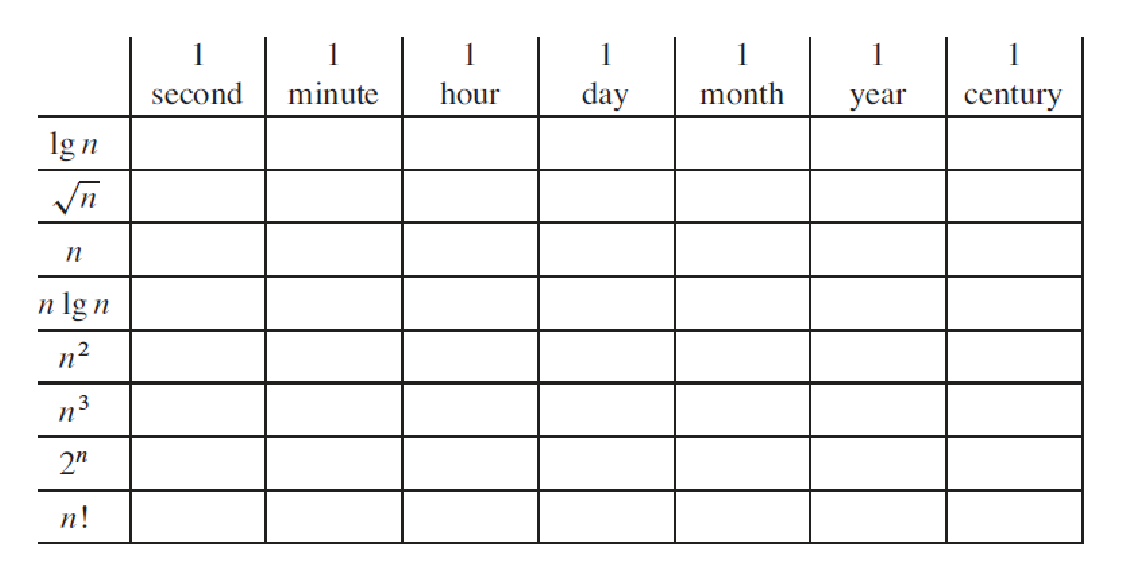
\includegraphics[scale=0.5]{fig/tableEksekusi.eps}%
\end{figure}
\end{konsep}

\subsection{Flow Chart}
Selain dengan menggunakan pseudocode, bisa juga menggunakan \textit{flow chart} untuk mengvisualisasikan sebuah algoritma. Bentuk dari \textit{flow chart} untuk algoritma \ref{algo:bubble} bisa dilihat di gambar \ref{fig:flowchart}.

\begin{marginfigure}%
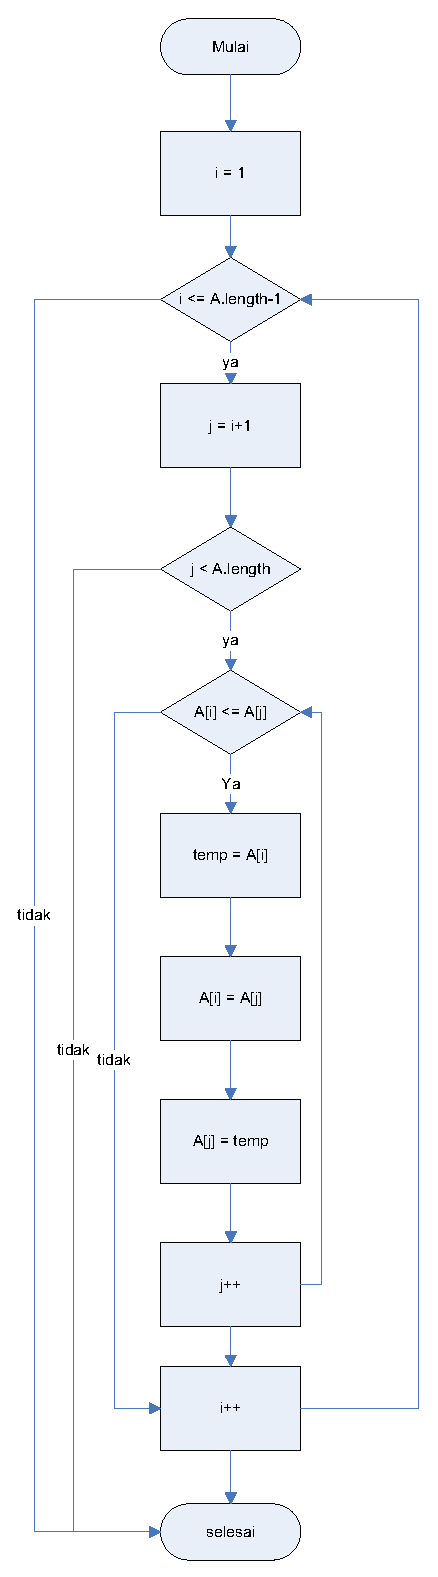
\includegraphics[scale=0.6]{fig/flowchart.eps}%
\caption{Flow Chart Bubble Sort}%
\label{fig:flowchart}%
\end{marginfigure}

\section{Implementasi algoritma ke bahasa pemrograman}
Algoritma \ref{algo:bubble} tidak bisa dijalankan secara langsung tanpa diimplementasi terlebih dahulu ke bahasa pemrograman. Bahasa yang digunakan di Algoritma \ref{algo:bubble} disebut sebagai \textit{pseudocode}. \textit{Pseudocode} sendiri tidak memiliki sebuah standar dalam penulisannya (tidak seperti bahasa Python yang memiliki aturan penulisan/sintaks). Penggunaan \textit{pseudocode} bisa berbeda-beda tergantung pada pembuat/penulisnya. 

Contoh implementasi Algoritma \ref{algo:bubble} ke bahasa pemrograman (Python) bisa dilihat di Listing \ref{lst:bubbleSortSimple}. Perlu diketahui, terdapat beberapa perbedaan mendasar antara algoritma dan listing program (misalnya indeks di algoritma dimulai dari 1 sedangkan di bahasa Python dimulai dari 0). 

\begin{listprog}{bubbleSort.py}
	\label{lst:bubbleSortSimple}
	\begin{lstlisting}[language=Python]
		A = [4,1,3,5,6,7,2]
		for i in range(1,len(A)):
				for j in range(i+1):
						if A[i]<=A[j]:
								temp = A[i]
								A[i] = A[j]
								A[j] = temp
		print A
	\end{lstlisting}
\end{listprog}

\section{Konsep dasar algoritma dan pemrograman}

\subsection{Variabel}

Variabel merupakan tempat penyimpanan data. 
\begin{contoh}
	\textbf{Penggunaan variabel}\\
	$a = 5 \rightarrow$ Memasukkan nilai 5 ke variabel `$a$'.\\
	$b = 7 \rightarrow$ Memasukkan nilai 7 ke variabel `$b$'.\\
	$a = b \rightarrow$ Memasukkan nilai variabel `$b$' ke variabel `$a$'. Kedua variabel sekarang bernilai 7.\\
	$a = b = 9 \rightarrow$ Memasukkan nilai 9 ke variabel `$a$' dan `$b$'.\\
\end{contoh}
\marginnote[-4cm]{
\begin{konsep}
Jika terdapat 4 variabel, yaitu: a, b, c, dan d dengan nilai a = 1, b = 2, c = 3, dan d =  4. Tuliskan sebuah algoritma untuk menukarkan isi variabel tersebut sehingga nilainya menjadi b = 1, c = 2, d = 3, dan a = 4. Usahakan agar pertukarannya minimum.
\end{konsep}}


\FloatBarrier
\subsection{Array}
Array\sidenote{Di bahasa pemrograman Python, implementasi dari Array disebut sebagai List.} merupakan kumpulan dari variabel. Satu array bisa menampung beberapa data. Gambar \ref{fig:illustrasiArray} menunjukkan illustrasi dari sebuah array yang berkapasitas $j$.
\begin{center}
	\begin{figure}[htbp]%
		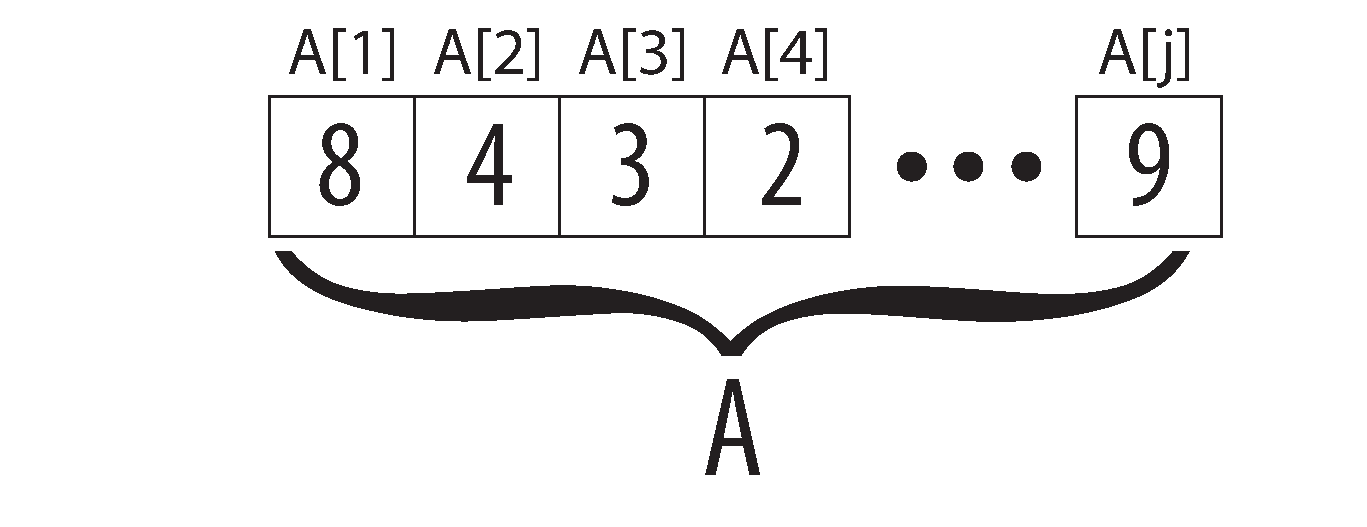
\includegraphics[scale=0.4]{fig/Array.eps}%
		\caption{Illustrasi Array}%
		\label{fig:illustrasiArray}%
	\end{figure}
\end{center}
\begin{contoh}
	\textbf{Penggunaan array}\\
	$A[i] \rightarrow$ Mengakses lokasi ke $i$ dari array yang bernama $A$.\\
	$A[4] \rightarrow$ Mengakses lokasi ke $4$ dari array yang bernama $A$.\\
	$A[i..j] \rightarrow$ Menandakan kumpulan isi array $A$ yang terdiri dari elemen $A[1],\ A[2],\ A[3],\ \ldots,\ A[j]$.\\
	$A[4] = 5 \rightarrow$ Memasukkan nilai 5 ke lokasi ke 4 dari array $A$.\\
	$b = A[4] \rightarrow$ Memasukkan nilai lokasi ke 4 dari array $A$ ke variabel $b$. 
	$A.length \rightarrow$ Menandakan besar/panjang dari array $A$.
\end{contoh}

\begin{pemrograman}
Lakukan langkah-langkah berikut di rumah:
\begin{enumerate}
	\item Unduh Python di \url{http://python.org/download/}.
	\item Pilihlah python versi 2.7.x yang sesuai dengan OS yang dipakai (Windows 32-bit---Python 2.7.3 Windows Installer, dan Windows 64-bit---Python 2.7.3 Windows Installer). Untuk Linux, python sudah secara \textit{default} terinstall (versi python tergantung dari distro linux yang digunakan).
	\item Install Python Installer yang sudah diunduh.
	\item Unduh IDE \textit{Integrated Development Environment} Python yang bernama PyScripter di \url{http://code.google.com/p/pyscripter}.
	\item Install PyScripter.
	\item Ketikkan Listing \ref{lst:bubbleSortSimple} dan jalankan.
\end{enumerate}
\end{pemrograman}

\begin{pemrograman}
Untuk melakukan latihan pemrograman algoritma dan Python di rumah, SPOJ merupakan website yang sangat berguna. SPOJ merupakan sebuah website \textit{Online Judge} dimana kita bisa melihat permasalahan-permasalahan yang menarik, menyelesaikan permasalahan tersebut dan meng-\textit{submit} solusinya ke SPOJ untuk di-\textit{judge}. SPOJ akan menentukan apakah solusi kita tepat atau salah. Diharapakan agar mahasiswa bisa menyelesaikan permasalahan SPOJ sebanyak mungkin untuk meningkatkan kemampuan pemrograman. Berikut langkah-langkah yang harus dilakukan di rumah.
\begin{enumerate}
	\item Buka website SPOJ (\url{www.spoj.pl})
	\item Register di website SPOJ tersebut.
	\item Baca tutorial di website SPOJ untuk memahami lebih lanjut di \url{http://www.spoj.pl/tutorials/}
	\item Lihat daftar permasalahan (\textit{problems}) di website SPOJ di \url{http://www.spoj.pl/problems/classical}
	\item Lihat permasalahan yang paling sederhana, yaitu permasalahan nomor 1 dengan CODE ``TEST'', atau dengan nama ``Life, the Universe, and Everything'' (\url{http://www.spoj.pl/problems/TEST/}).
	\item Baca dan coba pahami soalnya.
	\item Untuk percobaan akan dikasihkan solusinya sebagai berikut dalam bentuk \textit{source code} Python. 
	\begin{listprog}{TEST.py}
	\label{lst:TEST}
	\begin{lstlisting}[language=Python]
		k=input()
		while k!=42:
			print k
		k=input()
	\end{lstlisting}
	\end{listprog}
	\item Submit solusi tersebut di \url{http://www.spoj.pl/submit/}, pastikan pilihan \textbf{Language} adalah Python (python 2.7) dan Problem code adalah TEST.
	\item Lihat hasilnya di \url{http://www.spoj.pl/status/} dan cari username anda di kolom USER. Jika ada tulisan ``accepted'' berarti anda telah berhasil menyelesaikan permasalahan tersebut. Jika tidak cek kembali apakah ada yang salah di langkah sebelumnya.
\end{enumerate}
\end{pemrograman}
